\chapter{Teori}\label{Teori}

\section{Trafik Model}

Til dette projekt har vi valgt at arbejde med emnet trafik og simulering, mere specifikt simulering af trafik. Vi agter altså at løse et problem inde for dette område hvor i vores fokus ligger på at lave en simulering der kan hjælpe med til at konstruere og udspille forskellige scenarier der kan udspille sig i traffikerede områder og på den måde også simulerer alternativer. Derfor har gruppen valgt at udarbejde en model der beskriver gruppens fælles definition på trafik. Formålet med dette er at have en model at arbejde med og inddrage i programmet der fungerer som produktet i dette projekt.

OBS: Dette afsnit er ikke færdigt og modellen kan og vil med høj sandsynlighed ændre sig igennem projektet af forskellige årsager! 

\subsection{Trafik Flow}

Trafik fænomener har i langt tid ikke været nemt at regne på. En publikation fra 1988 af Paul Ross fra Traffic Systems Division beskriver trafik som at have en vis lighed med væsker som ikke kan komprimeres mere end en vis densitet \cite{trafdyn}. Igennem tiden har der været nogle forskellige teorier om hvorvidt man måler på trafik og mange har forsøgt på forskellige måder. 

%En publikation fra 1988 af en Paul Ross fra Traffic Systems Division, belyser om emnet Traffic Dynamics og herunder Traffic Flow \cite{trafdyn}. Som Paul Ross beskriver så området et af dem der er mindst forstået da der på dette tidspunkt ikke var nogle kontinuum teorier der kunne forudse trafik densitet, volume og fart med den præcision som der forventes for at kunne opstille et timing signal. Derimod er det bedste der kan gøres er at lave et cirka estimate med diskontinuerlig dellinger[Ordliste]. Publikationen forklarer i større detalje hvordan at for at få et udbytte med kontrol, simulation og en general forståelse for emnet, er en beskrivelse af trafik med henhold til fortsættende og differentiable kvantitativer[Ordliste] nødvendig. Formålet med denne publikation er at udvikle en ny formulering til dette som er kvalitativt korrekt. 

Den generelle konsensus for trafik variabler er følgende: Trafik Densiteten, K, farten, v, og volume, Q, er passende og brugbare til formået beskrevet herover. [Note: Cite Dr. Henry Lieu]


\[Q = Kv \]\label{eq:Equation1}\begin{flushright}(1)\end{flushright}
						
hvor følgende er gældende:

Q = trafik flow (Bil(er)/timen) forbi et punkt.  
K  = vehicular densitet (bil(er)/km)
v  = (space-mean-speed) fart (km/t)

Densitet kan beskrives som antallet af fartøjer per længden af en enhed (i dette tilfælde km). De to vigtige former af densitet er kritisk densitet, K\_c og jam densitet, K\_j. K\_c er den maksimale densitet under free flow. k\_j er den maksimale densitet under ophobning. Densitet udregnes som:

\[ k = \frac{1}{s} \]\label{eq:Equation2}\begin{flushright}(2)\end{flushright}

Hvor s er det inverse af densiteten, spacing, som er distancen fra midte til midte mellem fartøjer.

På en vej L vil densiteten K, på et bestemt tidspunkt t\_1, være lig det inverse af spacing mellem n antal fartøjer.

\[ K(L,t_1) = \frac{n}{L} = \frac{1}{\overline{s}(t_1)} \]\label{eq:Equation3}\begin{flushright}(3)\end{flushright}

Space-mean-speed kan forklares som at være en udregning af fart hvori man tager et helt vejbane segment i betragtning. En serie af billeder eller video optager farten på individuelle fartøjer der køre på denne bane, ud fra dette er en gennemsnits fart udregnet. Denne type udregning anses for at være mere præcis end Time-mean-speed metoden som der ikke vil blive forklaret i dette afsnit. Udregningen vor Space-mean-speed ser således ud:

\[ v_t = n (\displaystyle\sum_{i=1}^{n}(1/v_i)^-1 \]\label{eq:Equation4}\begin{flushright}(4)\end{flushright}

Hvor n er det antal af fartøjer der passere vejbane segmentet.

\subsection{Flow}
Flow er det antal at fartøjer som passere en form for referrence punkt per enhed af tid, som fartøjer/timen. The inverse af flow er togfølge (h) hvilket er den tid der går imellem fartøjer der passere det bestemte punkt og det forrige køretøj (i + 1). Ved overbelastning på veje forbliver h constant. Ved en trafik prop vil h gå mod uendeligt.

\[ q = 1/h \]\label{eq:Equation5}\begin{flushright}(5)\end{flushright}

Flow (q) der passere et bestemt punkt (x\_1) i et interval (T) er lig det inverse af den gennemsnitlige togfølge af m køretøjer.

\[ q(T, x_1) = \frac{m}{T} = \frac{1}{h(x_1} \]\label{eq:Equation6}\begin{flushright}(6)\end{flushright}

Lastbiler:
Lastbiler og andre transport fartøjer er oftest skyld i at trafikken går langsommere eller i nogle tilfælde stopper helt op. Det er derfor at bl.a. transport af vindmølledele bliver igangsat sent om aften eller meget tidligt på morgenen således at de ikke skaber problemer for andre billister. Dette har altså en stor effekt på trafikken og kunne derfor være relevant at medtage i vores model, dette er dog ikke gruppens fokus da dette er et meget specifikt scenarie.
NOTE: Kan ændres skulle vi have tid til at lave noget med denne type scenarie.

Tid på dagen / Rush Hour: 
Rush hour er det scenarie hvori der sker mest trafik i et land. Dette er typisk i de timer hvor de forskellige bilister skal på arbejde, køre børn til skole eller andre institutioner eller lignende og igen når disse samme individer skal hjem igen. Dette kan indskrives i programmet som en form for variable der ændre mængden af trafik ved bestemte tidspunkter.
NOTE: Mangler kilde på dansk rush hour.

\section{INTRO TIL TEORI, SKAL SÆTTES I LØSNINGSAFSNIT}
Til udformning af vores løsningsmodel bidrager dette afsnit en gennemang af to algoritmer til ruteplanlægning og vejvisning. De er valgt på baggrund af deres udbredthed i industrien (KILDE). TEKNOLOGIANALYSEN anleder til at afgøre hvilke(n) algoritme(r) der er nødvendige til vores løsningsmodel. Der er blevet valgt to algoritmer til vejvisning som er A* og Dijkstras Algoritme.
Der vil først blive gennengået deres generelle funktion og dernæst en sammenligning af de to og en videre afgrænsning til hvilken der vil blive benyttet til løsningsmodellen.

\vspace{5mm}

\section{A* Algoritmen}
Primært når det kommer til belægning af en dynamisk rute, foregår det ved at en enhed fortsætter hen i mod et mål indtil den når en forhindring. Dette er et ekstremt simpelt bevægelsesmønster og indebærer in vis in-effektivitet. Rent retorisk kunne man stille spørgsmålet om det ikke ville være smartere at planlægge en rute før man overhovedet bevæger sig.

\vspace{5mm}

A* er en algoritme til at beregne den korteste rute baseret på en række heuristiske datasæt. A* får input igennem en brugerlavet graf der indeholder en række datasæt for at algoritmen kan fungere.  Først har vi distancen fra punkt til punkt, eksempelvis punkt 'A' til punkt 'B' som vi kalder for f.eks. \textbf{H} og dernæst har vi et datasæt \textbf{G} der indeholder bekostningen for at flytte fra en kant til en anden, denne variabel er bestemt på forhånd. Et virkelighedseksempel kunne være at man vil over på den anden side af en sø, så har man så muligheden for at svømme direkte eller gå uden om og det koster f.eks. 2 gange så meget at bevæge sig direkte igennem søen. Dette er givet ved \textbf{G}, hvor som sagt \textbf{H} er den ultimative korteste længde til det bestemte slutpunkt. \textbf{H} fungerer desuden for hvilket som helst punkt i et system og angiver \textit{altid} den korteste vej til slutpunktet uanset forhindringer. Det skal også nævnes at \textbf{H} ikke er påvirket af bevægelsesbekostningen, til at starte med, som \textbf{G} angiver, dette kommer først senere. Til sidst har vi \textbf{F} der er en samenlagt værdi af både \textbf{H} og \textbf{G}. Dette gælder kun for hver kasse der flyttes til, hvori \textbf{H} er angivet ved kassen man flytter tils \textbf{H} værdi. Det kan vises således i formlen \ref{eq:A*}:
\begin{equation} \label{eq:A*}
F(n) = G(n) + H(n)
\end{equation}

En måde man kan visualisere A* på er f.eks. med et gitter-system som set i figur \ref{fig:AKvadrat1}. Her kan vi se at vi har et start punkt (grøn) og et slutpunkts (blå). De kasser vi ikke kan bevæge os igennem er de røde kasser. Figuren angiver ingen heuristiske datasæt endnu.

\begin{figure}[H]
\begin{adjustbox}{width=1.2\textwidth,center=\textwidth}
\centering
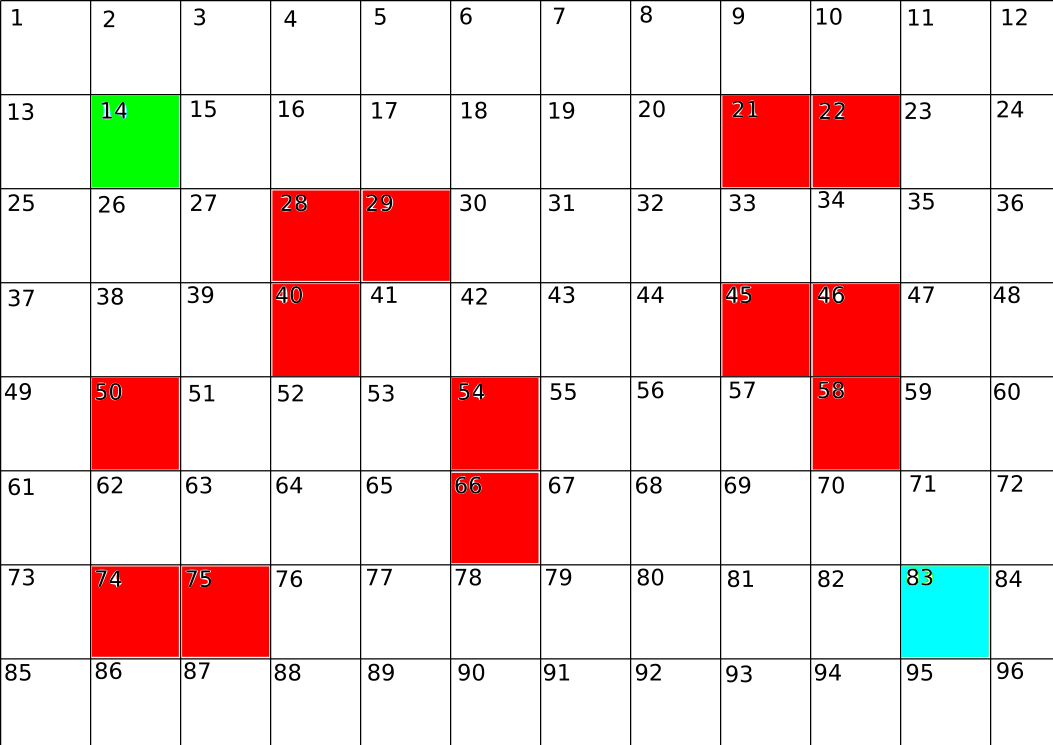
\includegraphics[width=1.2\textwidth]{Pictures/Teoriafsnit/Figurfiler/Grid2.png}
\end{adjustbox}
\caption{A* gitter-system}
\label{fig:AKvadrat1}
\end{figure}

Ud fra figuren kan vi begynde os at forestille hvordan A* fungerer. Når man bevæger sig fra kasse til kasse laver man 2 lister til at holde styr på hvor brikken har været. En liste til at holde styr på hvilke kasser man ikke har besøgt endnu og en liste der holder styr på hvilke man \textbf{har} besøgt. Når man flytter brikken skal man derfor angive hvilken kasse der nu skal på \textit{besøgt} listen. Derfor som nævnt skal vi bruge information om hvor meget \textbf{G} koster. Brikken skal nu til at flytte sig for at komme til slutpunktet. Dette kunne f.eks. være 10 point for at flytte sig i hvilken som helst retning, men man kunne også sagtens angive at diagonal bevægelse ville koste 12 point. Dvs. at ruten ændrer sig til måske ikke at være så direkte som den ellers kunne have været.

\vspace{5mm}

Der findes flere metoder man kan anvende A* på og en af dem vises her.
Det vises her i den lille bid af Python-kode i Listing \ref{lst:Apseudo1}:
\begin{lstlisting}[caption={A stjerne og pseudo-kode af brug af lister},label={lst:Apseudo1},language=C]
frontier = Queue()
frontier.put(start)
visited = {}
visited[start] = True

while not frontier.empty():
   current = frontier.get()
   for next in graph.neighbors(current):
      if next not in visited:
         frontier.put(next)
         visited[next] = True
\end{lstlisting}
\cite{stanfordredblobgamesAstar}

Som set i figur \ref{fig:AKvadrat1} har vi vores liste givet ved kassernes nummerering. Nummereringen kører fra venstre mod højre én række ad gangen. Vi angiver at det tager 10 point af gå lodret og vandret én kasse ad gangen og 12 point at gå diagonalt. I figur \ref{fig:AKvadrat2} kan vi nu se de heuristiske datasæt angivet fra startpunktet (grøn). Hver enkel kasse omkringliggende startpunktet har deres \textbf{H} værdi angivet med lys-lilla tekst og bevægelsesomkostningen \textbf{G} fra startpunktet til kassen angivet i blå tekst.

\begin{figure}[H]
\begin{center}
\includegraphics[width=1.00\textwidth]{Pictures/Teoriafsnit/Figurfiler/Grid3.png}
\end{center}
\caption{A* der viser bekostning af bevægelse fra startpunkt (grøn) til omkringliggende kasser (G) angivet med blå farve samt H angivet med lys-lilla}
\label{fig:AKvadrat2}
\end{figure}

Nu udregnes \textbf{F} værdien så f.eks. hvis vi går fra kasse 14 (startpunktet) til 15 skal vi lægge 10 (\textbf{G}) og 8 (\textbf{H}) sammen. Dette gør vi så for alle omkringliggende kasser for startpunktet. Dernæst går man til den laveste \textbf{F} værdi og gør helt det samme som før, derudover flyttes den nye kasse man står på til \textit{besøgt} listen. Noget man skal være opmærksom på her er at man stadig skal sammenligne bevægelsesomkostningen fra den tidligere kasse til de kasser der også er relevante for den nye kasse man har flyttet sig til. For dermed at afgøre om man kunne have påført en smartere bevægelse. Det skal igen pointeres at A* modtager data fra en graf og det her modelleres.

\vspace{5mm}

Denne fremgangsmåde er også bedre kendt som Breadth First Search, hvori en frontlinje bliver kontinuerligt fremskyndet baseret på omkostninger og heuristiske datasæt\cite{stanfordredblobgamesAstar}.
A* er en heuristisk fremgangsmåde afledt af Dijkstras generelle funktionalitet. Dijkstra og A* vil altid give en kortest vej hen til målet.  %\cite{http://search.proquest.com/openview/88fa950a98b308c6687f79f76caeb187/1?pq-origsite=gscholar}

\section{Dijkstras Algoritme}

Dijkstras algoritme er en algoritme til at finde den korteste vej fra et bestemt punkt til et andet punkt. Disse punkter kan bland andet repræsentere den korteste vej mellem to forskellige byer. Dijkstra fungerer på nogenlunde samme måde som A* i dens planlæggende fremgangsmåde ved at sammenligne punkter med hinanden. Dijkstras algoritme skanner også et område af kasser fra et startpunkt og fortsætter som eksemplificeret i figur \ref{fig:AKvadrat2}. Dijkstra modtager dog ikke heuristiske datasæt Dijkstras er en grådig algoritme, da den finder den korteste længde først og fortsætter således.\cite{DMATBOGEN} Dette kaldes også Greedy Best First Search.

\vspace{5mm}

Dijkstras algoritme finder den korteste rute mellem 2 forskellige punkter i en simpel ikke-orienteret vægtet graf. Man kan se på figur \ref{fig:dijkstrasgraf} at der angives forskellige punkter {A, B, C, D, E, Z}. Hvis man skal fra punkt A til Z på figuren, så starter man ved A og derfor initialiseres A til at være 0, som man kan se på tabel \ref{fig:dijkstratabel}. Algoritmen virker således, at alle punkter er uendeligt udover det punkt man befinder sig på som vist på tabel \ref{fig:dijkstratabel}. Algoritmen tager punkt fra punkt, så den starter med at se de grene som A har. Disse er |AB| = 4 og |AC| = 2. Her fra kan algoritmen ikke se videre end B og C. Den ser altid på det mindste tal, og derfor tager den længden fra A til B som er 4 og længden fra A til C som er 2, begge disse tal er mindre end uendeligt. Herefter ser den efter hvilket af de nuværende tal som er mindst, hvilket er 2. Så derfor vælger den C som sit næste punkt. Algoritmen finder nu de næst tætteste punkt, ved at addere alle de tidligere ruter, som har den korteste rute fra A til det næste sæt af punkter. Her ser algoritmen ud fra C og hvilke grene C har. Dette er længden til B, D og E, dog er længden altid fra A, så derfor er længden fra A til E 12 da 2+10 = 12. Længden til B er nu blivet 3, da algoritmen ser på den korteste rute, så A til B er 3, da 2+1 = 3. Således fortsætter algoritmen indtil den rammer Z.\cite{DMATBOGEN}

\begin{figure}[H]
\begin{adjustbox}{width=1.2\textwidth,center=\textwidth}
\centering
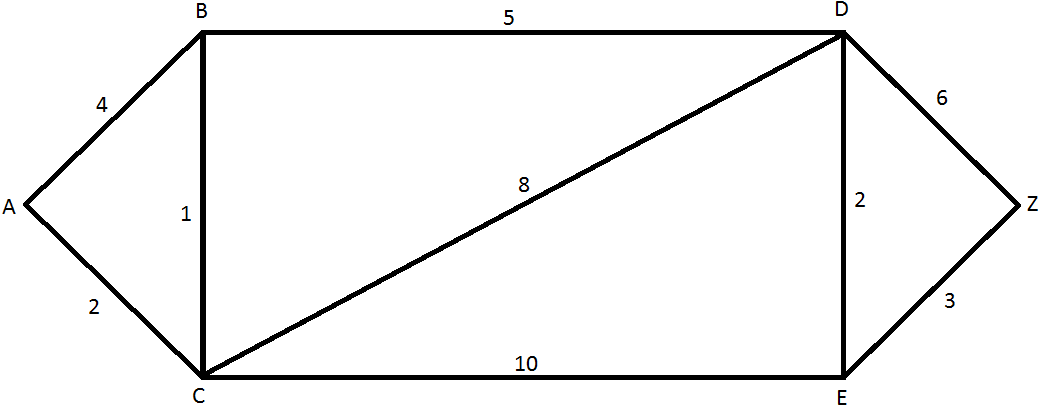
\includegraphics[width=1.2\textwidth]{Pictures/Teoriafsnit/Figurfiler/dijkstrasgraf.png}
\end{adjustbox}
\caption{Graf til fremvisning af eksempel af Dijkstras algoritme i brug}
\label{fig:dijkstrasgraf}
\end{figure}

\begin{table}[H]
\centering
\begin{adjustbox}{width=1\textwidth}
\Large
\begin{tabular}{| c | c | c | c | c | c | c |}
	\hline
	 & A & B & C & D & E & Z \\
	\hline
	 & 0 & Inf & Inf & Inf & Inf & Inf \\
	\hline
	{A} & 0 & 4 & 2 & Inf & Inf & Inf \\
	\hline
	{A, C} & 0 & 3 & 2 & 10 & 12 & Inf \\
	\hline
	{A, C, B} & 0 & 3 & 2 & 8 & 12 & Inf \\
	\hline
	{A, C, B, D} & 0 & 3 & 2 & 8 & 10 & 14 \\
	\hline
	{A, C, B, D, E} & 0 & 3 & 2 & 8 & 10 & 13 \\
	\hline
	{A, C, B, D, E, Z} & 0 & 3 & 2 & 8 & 10 & 13 \\
	\hline
\end{tabular}
\end{adjustbox}
\caption{Dijkstra tabel}\label{fig:dijkstratabel}
\end{table}

\begin{lstlisting}[language=C,caption={Dijkstras angivet som eksempel i pseudo-kode},label={lst:DijsktrasPseudo1}]
	procedure Dijkstras(G: weighted connected simple graph, with all weights positive)
{G has vertices a = V0, V1, ....... Vn = z and lengths w(Vi, Vj) where w(Vi,Vj) = infinity if{Vi, Vj} is not an edge in G}
for (i = 1 to n)
	L(Vi) = infinity
L(a) = 0
S = NULL
{ the labels are now initialized so that the label of a is 0 and all other labels are infinity, and S is the empty set }
while (z does not belong to S)
	u = a vertex not in S with L(u) minimal
	S = S U {u}
	for (all vertices v not in S)
		if (L(u) + w(u, v) < L(v) then L(v) = L(u) + L(u, v))
		{this adds a vertex to S with minimal label and updates the labels of vertices not in S}
return (L(z)) {L(z) = length of a shortest path from 	a to z}
\end{lstlisting}